  \documentclass{article}

\input{"MathTopMatter.tex"}

\usepackage[framed,numbered,autolinebreaks,useliterate]{mcode}

\usepackage{fullpage}

\title{Seperation of Video in Foreground/Background using DMD (AMATH 582 Homework 4)}
\author{Ronan Keane}
\date{4182 W Stephen's Way NE, Room 103, ~Seattle, WA 98105 \\ ~ronank@uw.edu~}

\makeatletter
\newcommand{\rmnum}[1]{\romannumeral #1}
\newcommand{\Rmnum}[1]{\expandafter\@slowromancap\romannumeral #1@}
\makeatother
%\renewcommand{\thesection}{Problem \arabic{section}.}
%\renewcommand{\thesubsection}{\arabic{section} (\alph{subsection})}
%\renewcommand{\thesubsubsection}{\arabic{section} (\alph{subsection}) (\roman{subsubsection})}

%\def\A{
%\begin{bmatrix}
%    x_1 & x_2 & \cdots & x_N
%\end{bmatrix}}

\begin{document}
\maketitle
%figures

\begin{figure}
	\centering
	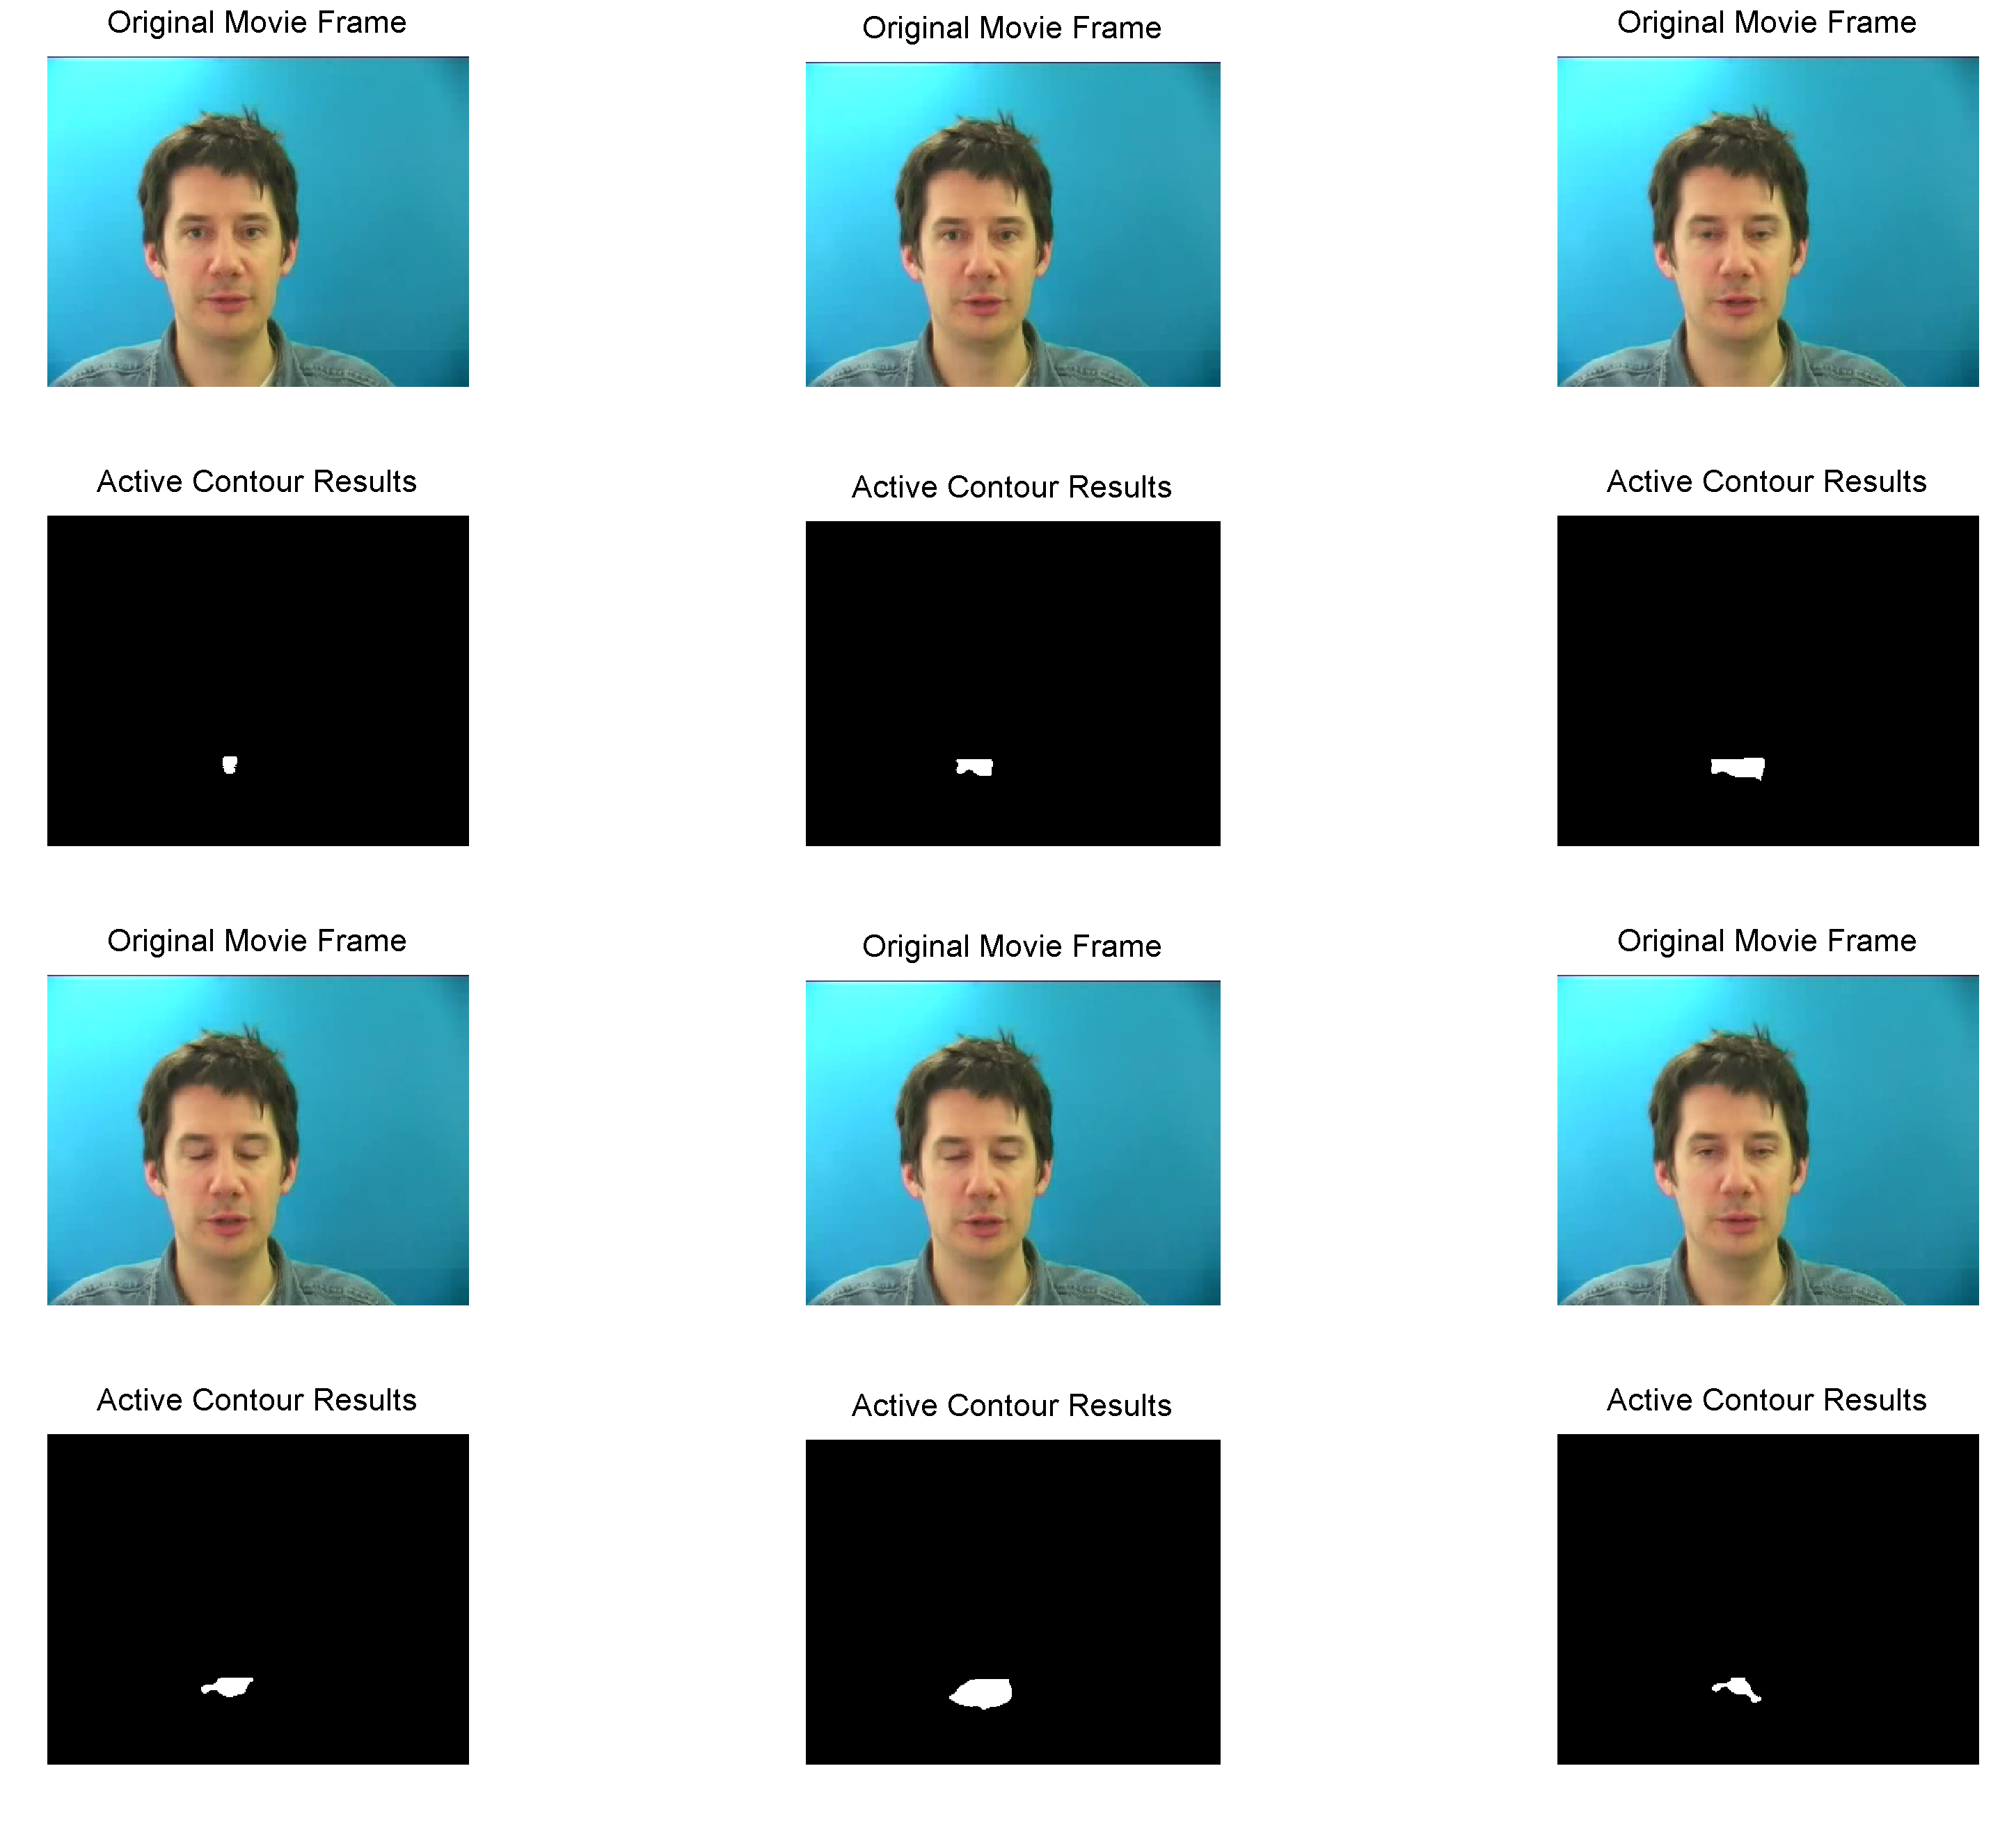
\includegraphics[width=1\textwidth]{AC1.png}
	\caption{Active Contour Results for selected frames. Active contour provides an inconsistent lip profile because it never properly converges.}
\end{figure}

\begin{figure}
	\centering
	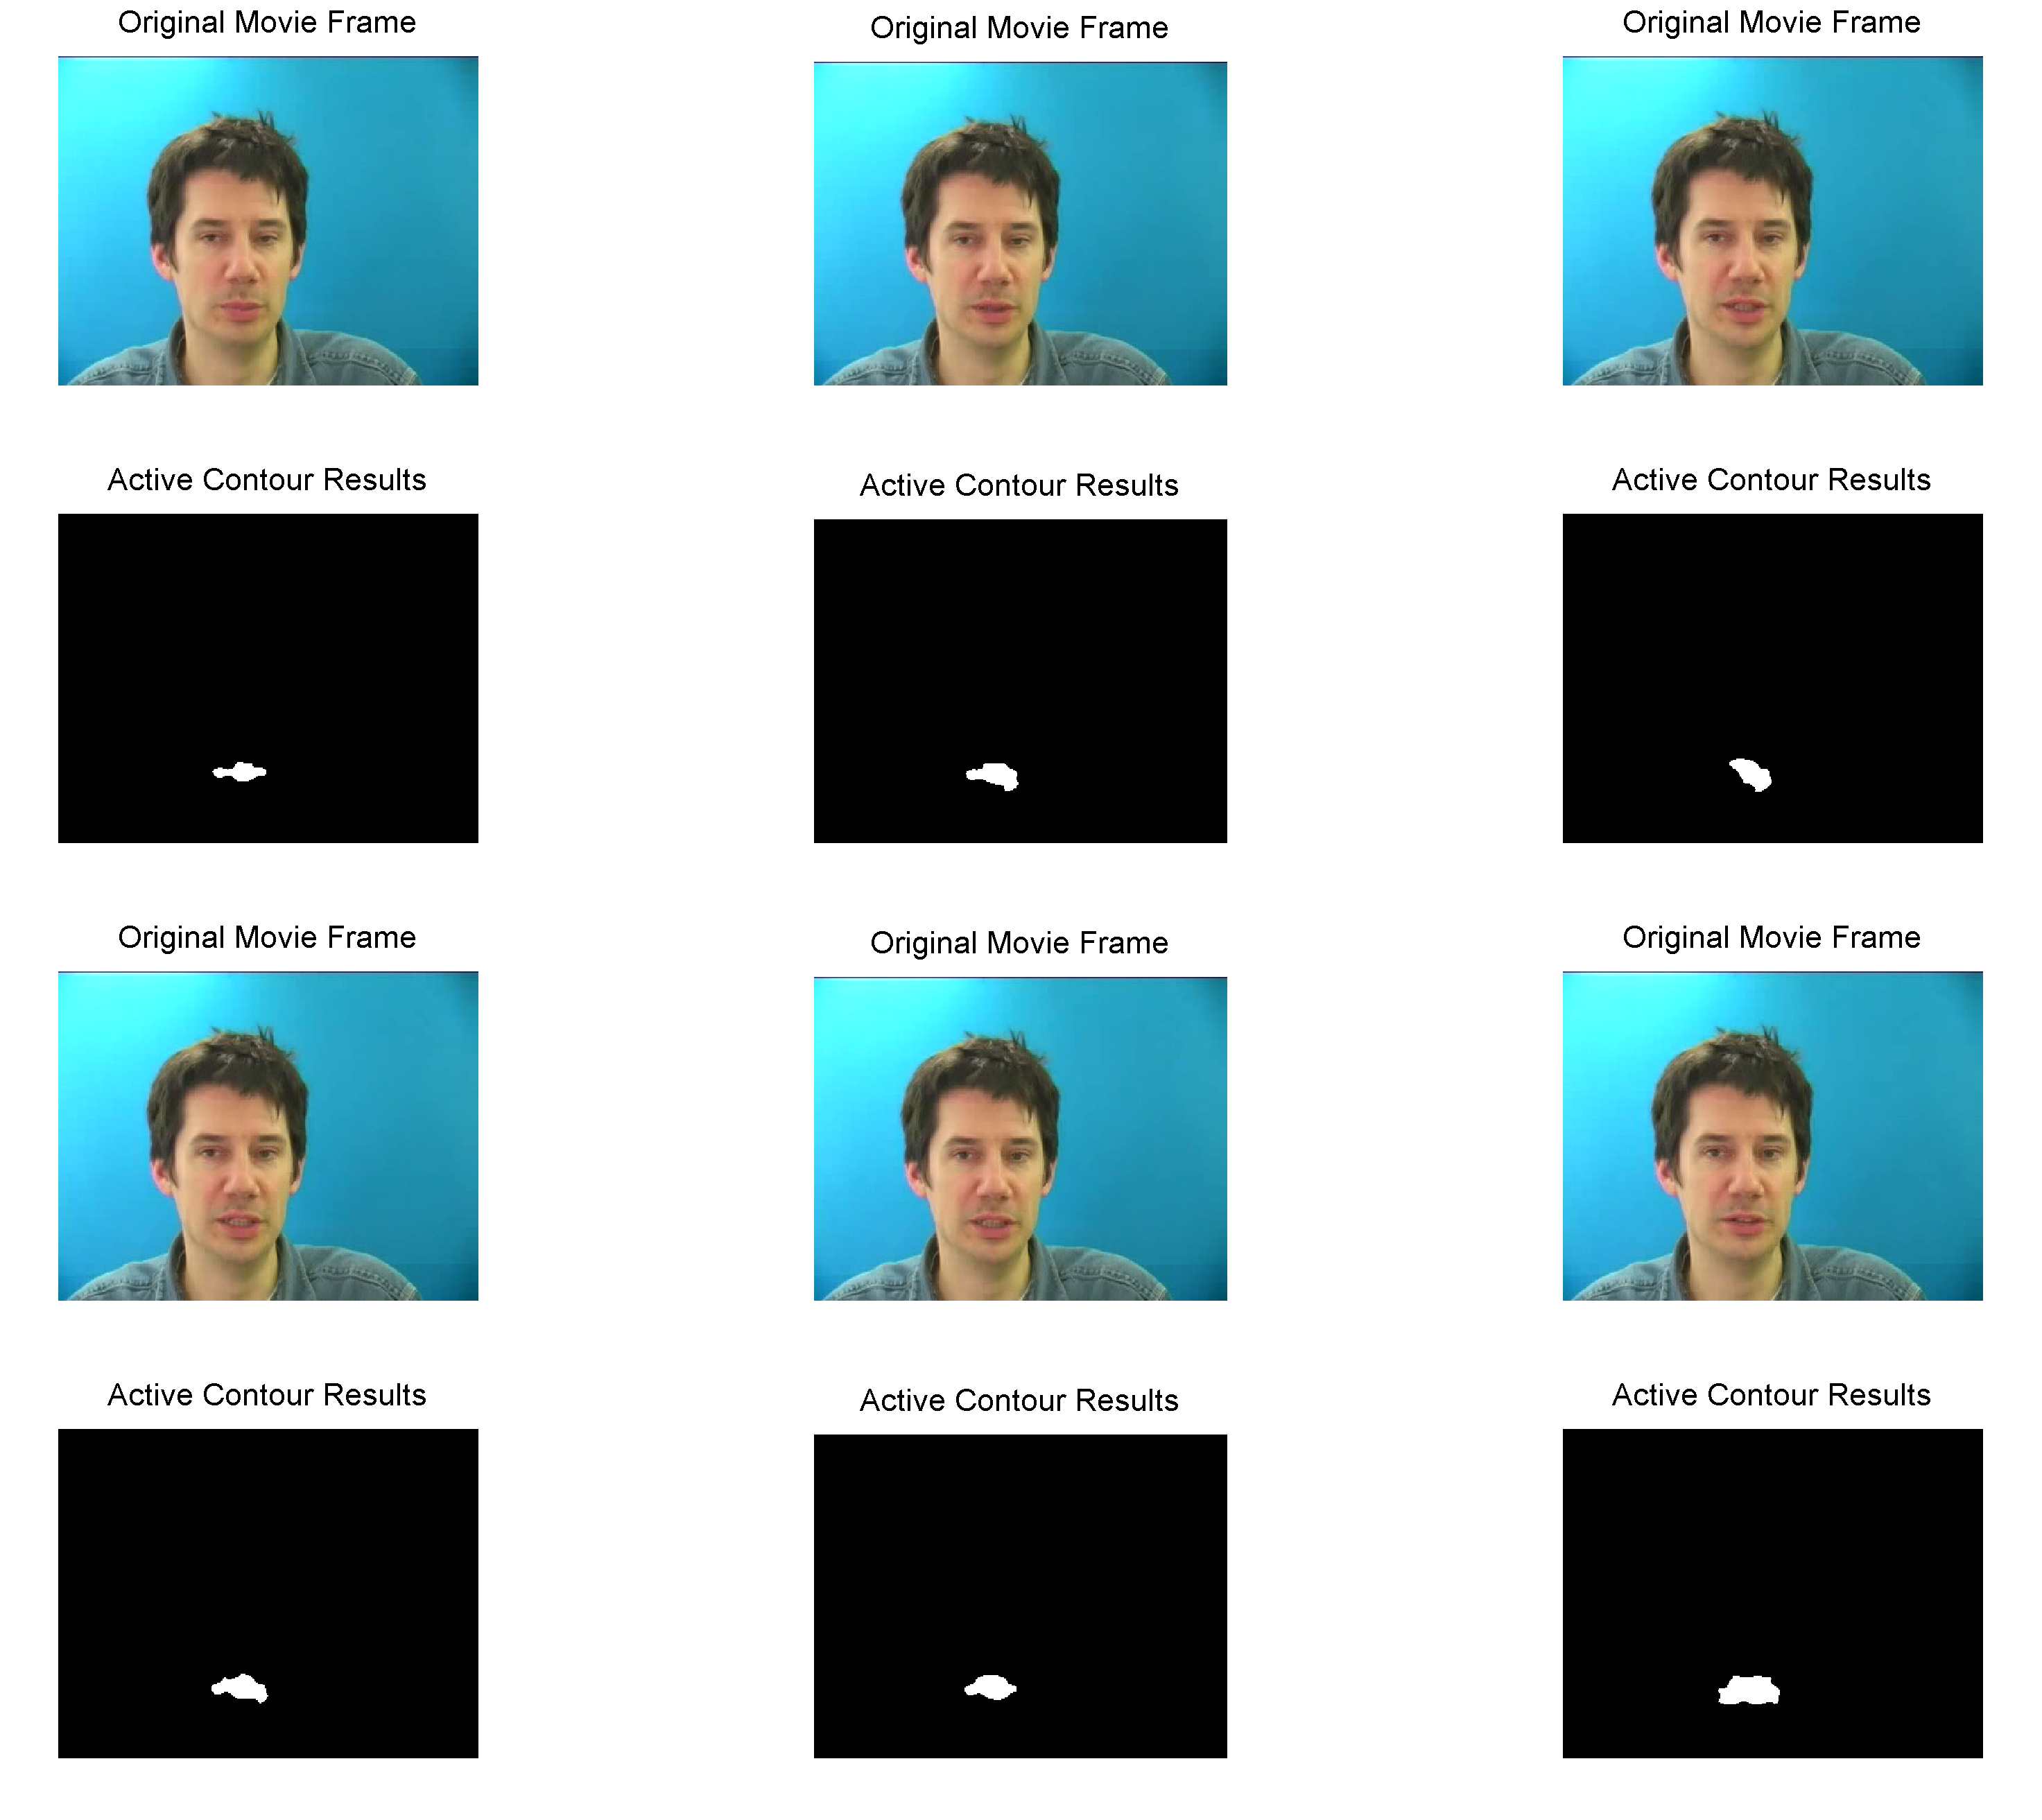
\includegraphics[width=1\textwidth]{AC2.png}
	\caption{Active Contour Results for selected frames. Active contour provides an inconsistent lip profile because it never properly converges.}
\end{figure}

\begin{figure}
	\centering
	\includegraphics[width=1\textwidth]{DMD1.png}
	\caption{DMD results for selected frames. DMD is not ideal in this situation because the background (the man's face) is not completely stationary.}
\end{figure}

\begin{figure}
	\centering
	\includegraphics[width=1\textwidth]{DMD2.png}
	\caption{DMD results for selected frames. DMD is not ideal in this situation because the background (the man's face) is not completely stationary.}
\end{figure}

\begin{figure}
	\centering
	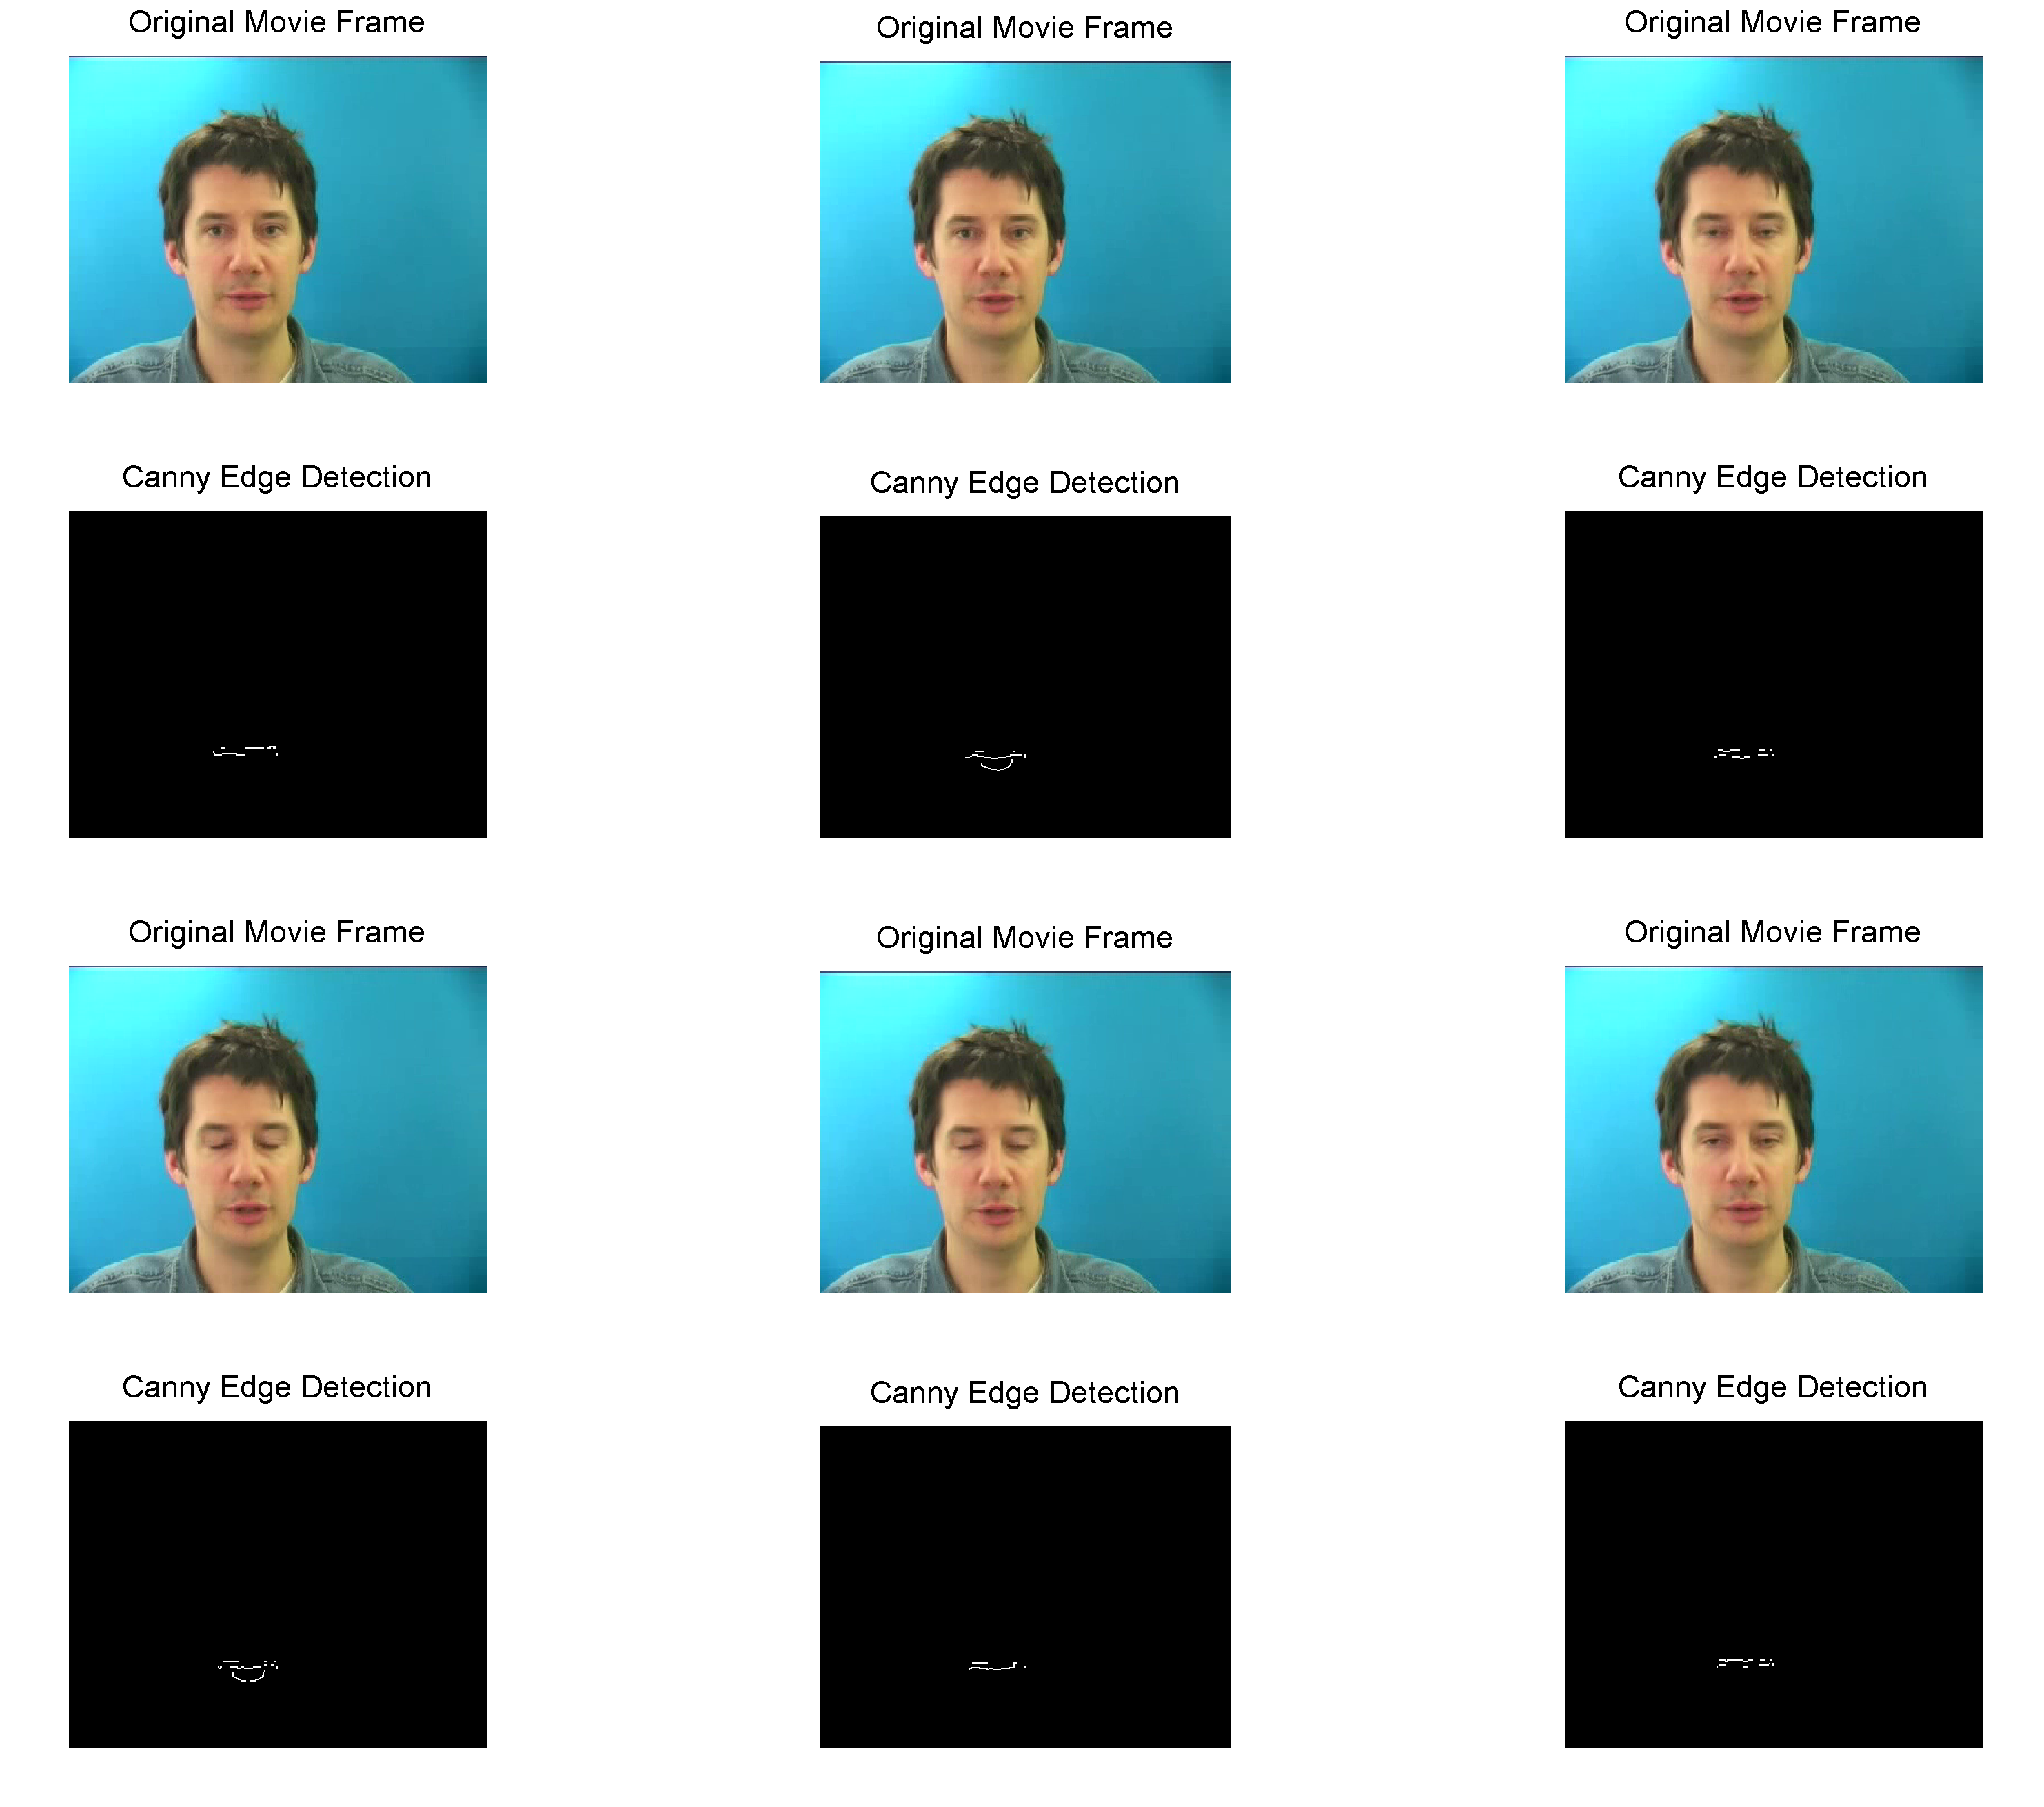
\includegraphics[width=1\textwidth]{canny1.png}
	\caption{Canny Edge Detection results for selected frames. Although it captures the profile of the lips, it does not always capture the entire contour.It also does not show the inside of the lips.}
\end{figure}

\begin{figure}
	\centering
	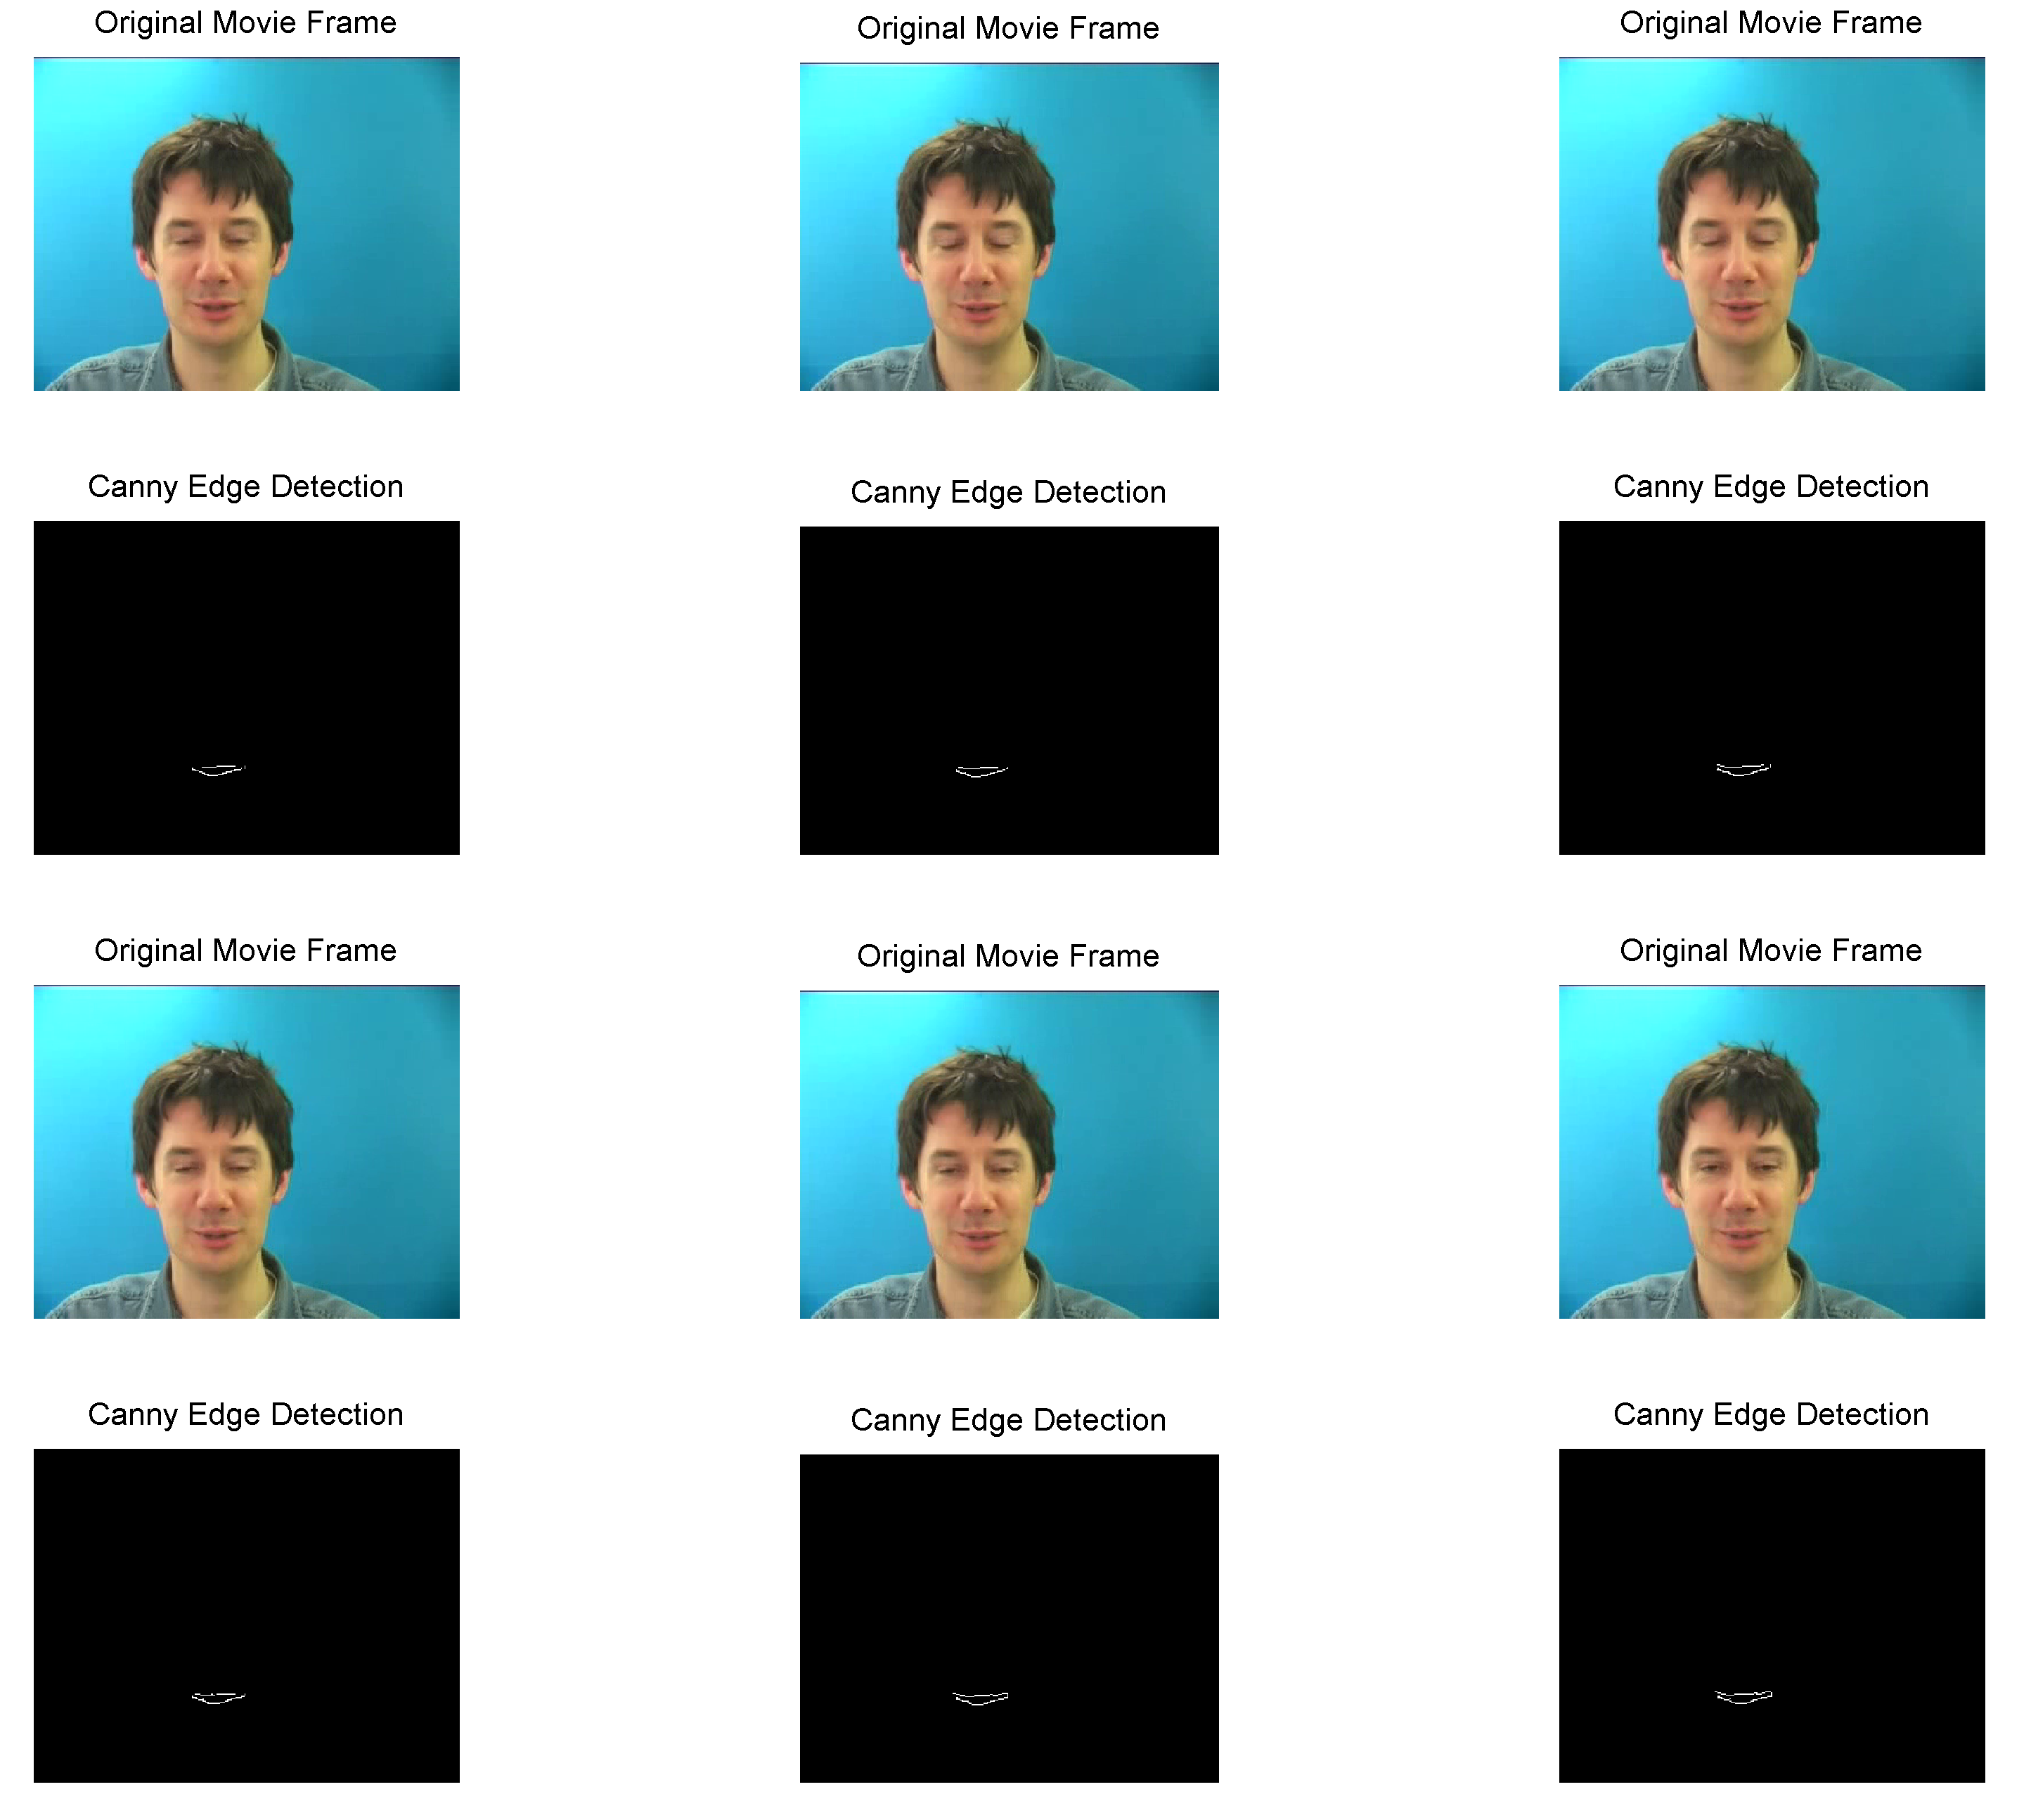
\includegraphics[width=1\textwidth]{canny2.png}
	\caption{Canny Edge Detection results for selected frames. Although it captures the profile of the lips, it does not always capture the entire contour. It also does not show the inside of the lips.}
\end{figure}

\begin{figure}
	\centering
	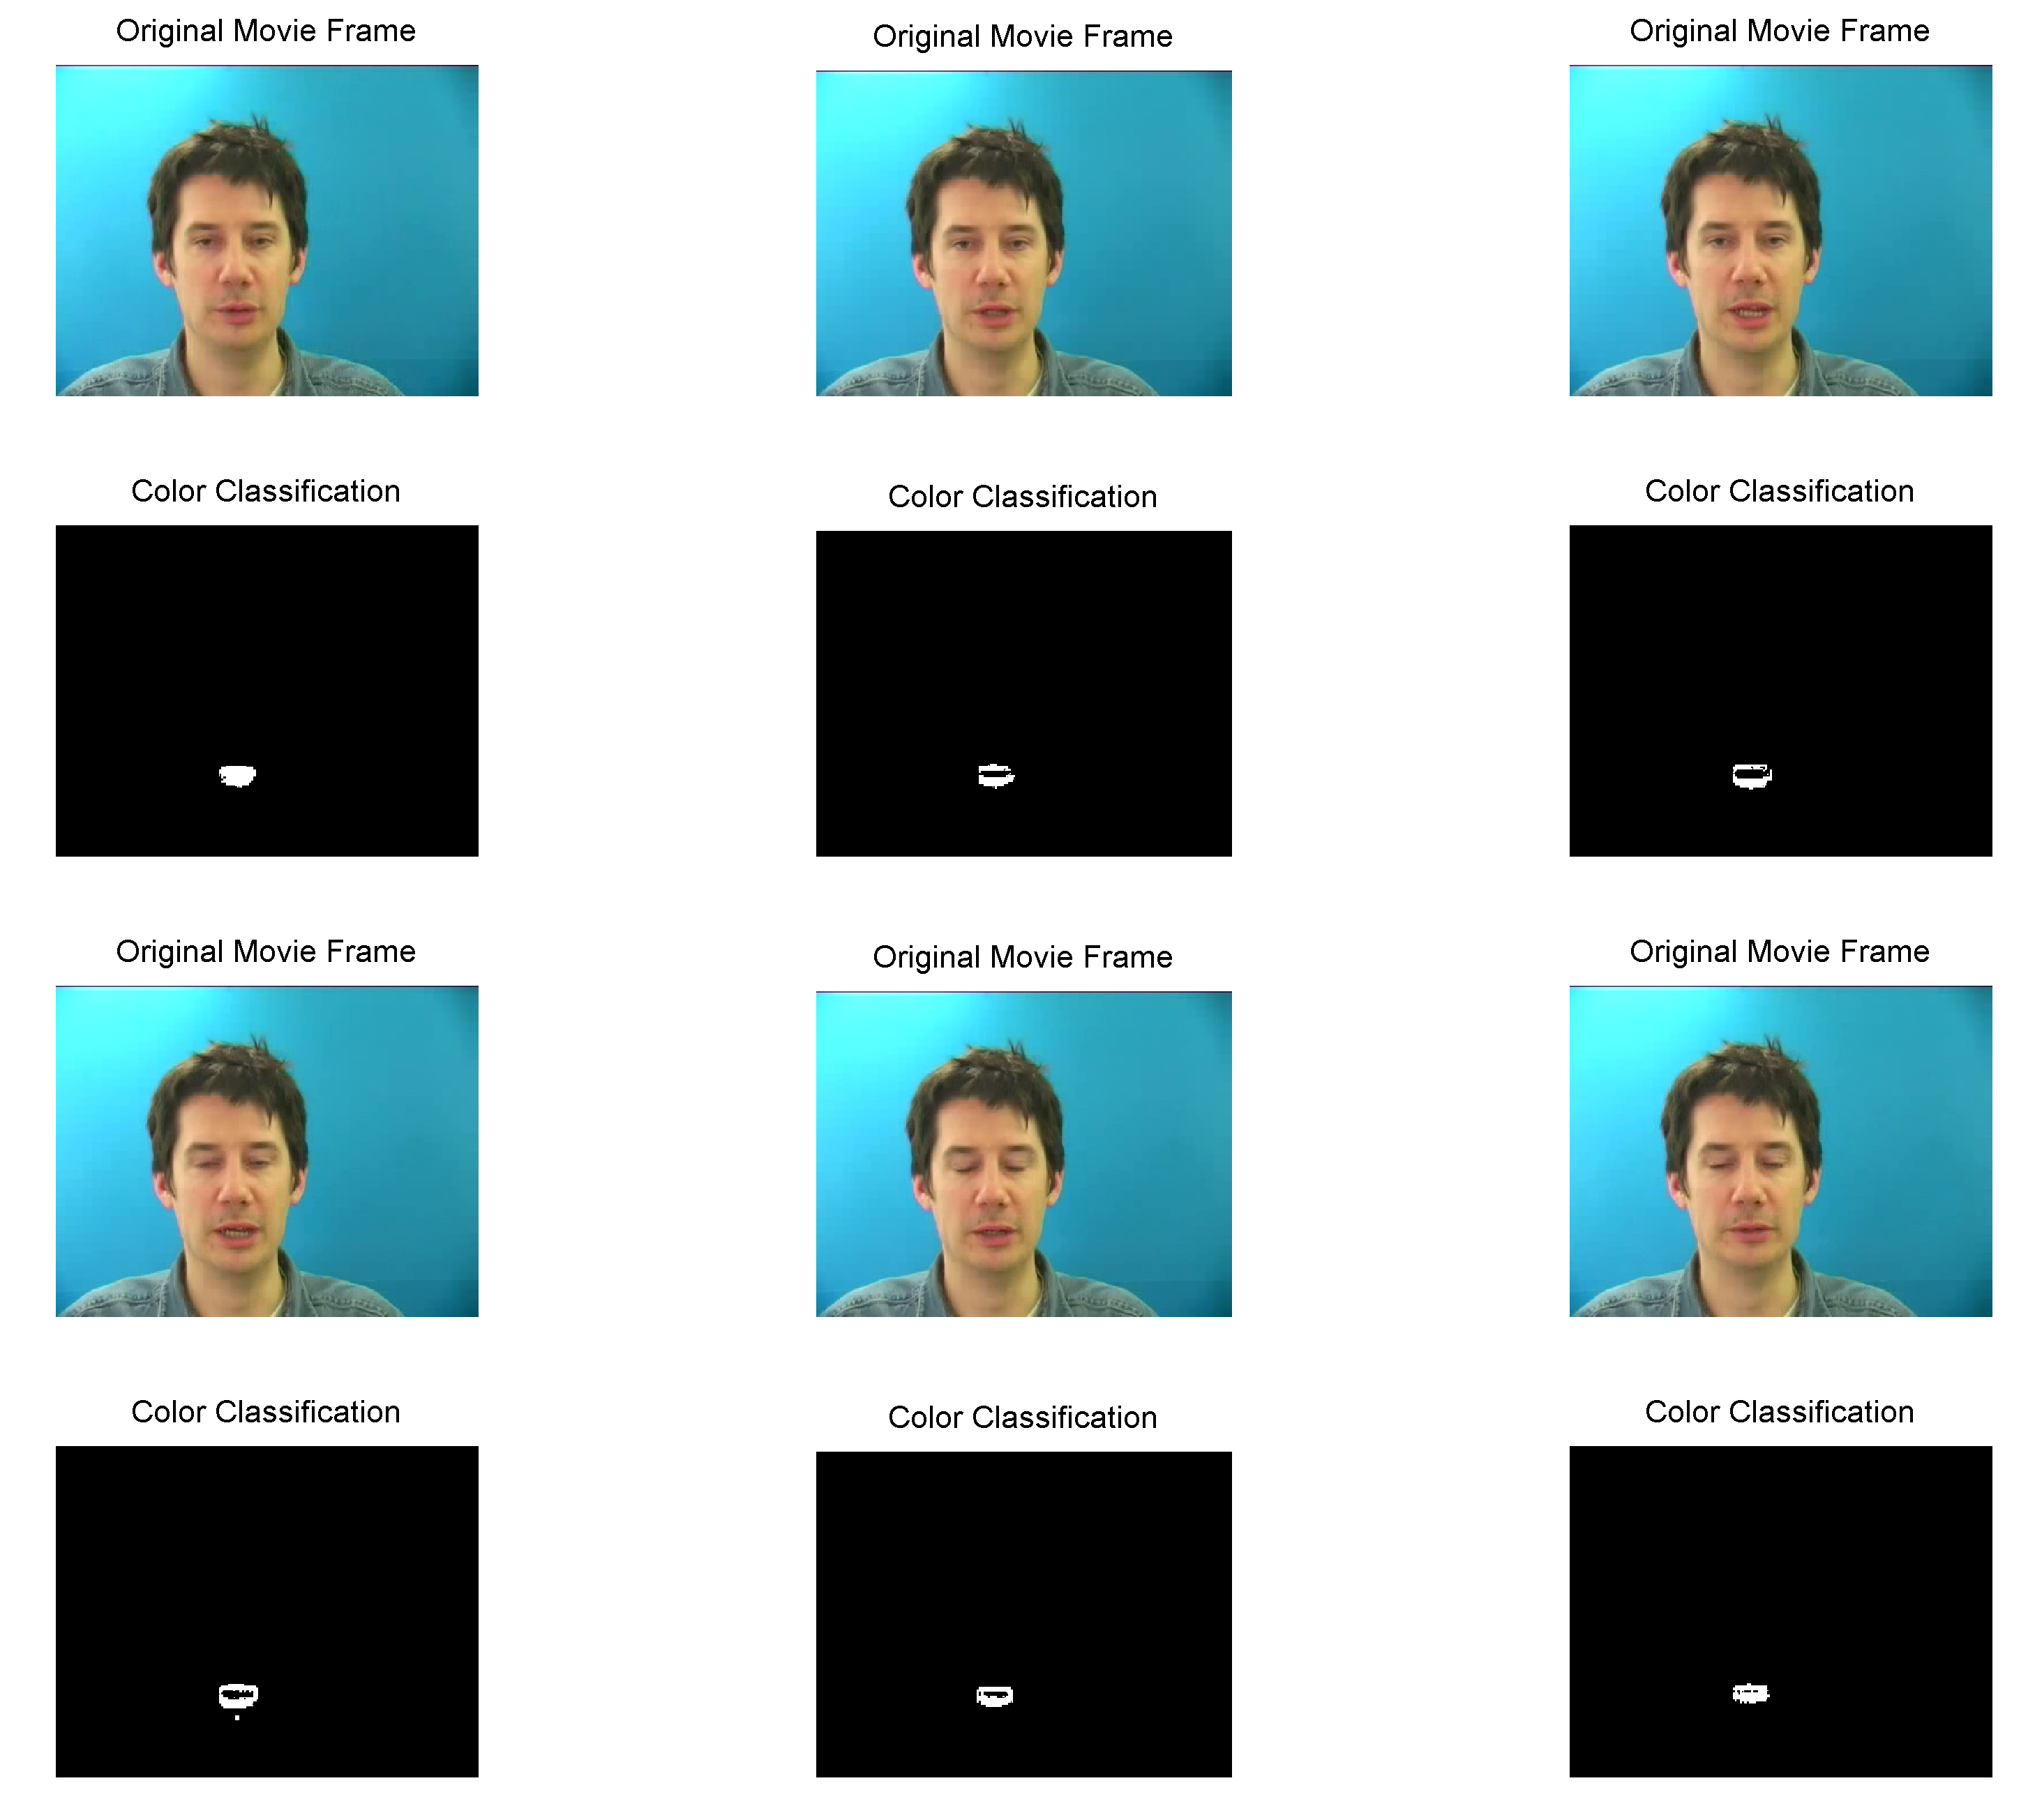
\includegraphics[width=1\textwidth]{color1.png}
	\caption{Color Classification for selected frames. Arguably the best overall method for capturing the movement of the lips.}
\end{figure}

\begin{figure}
	\centering
	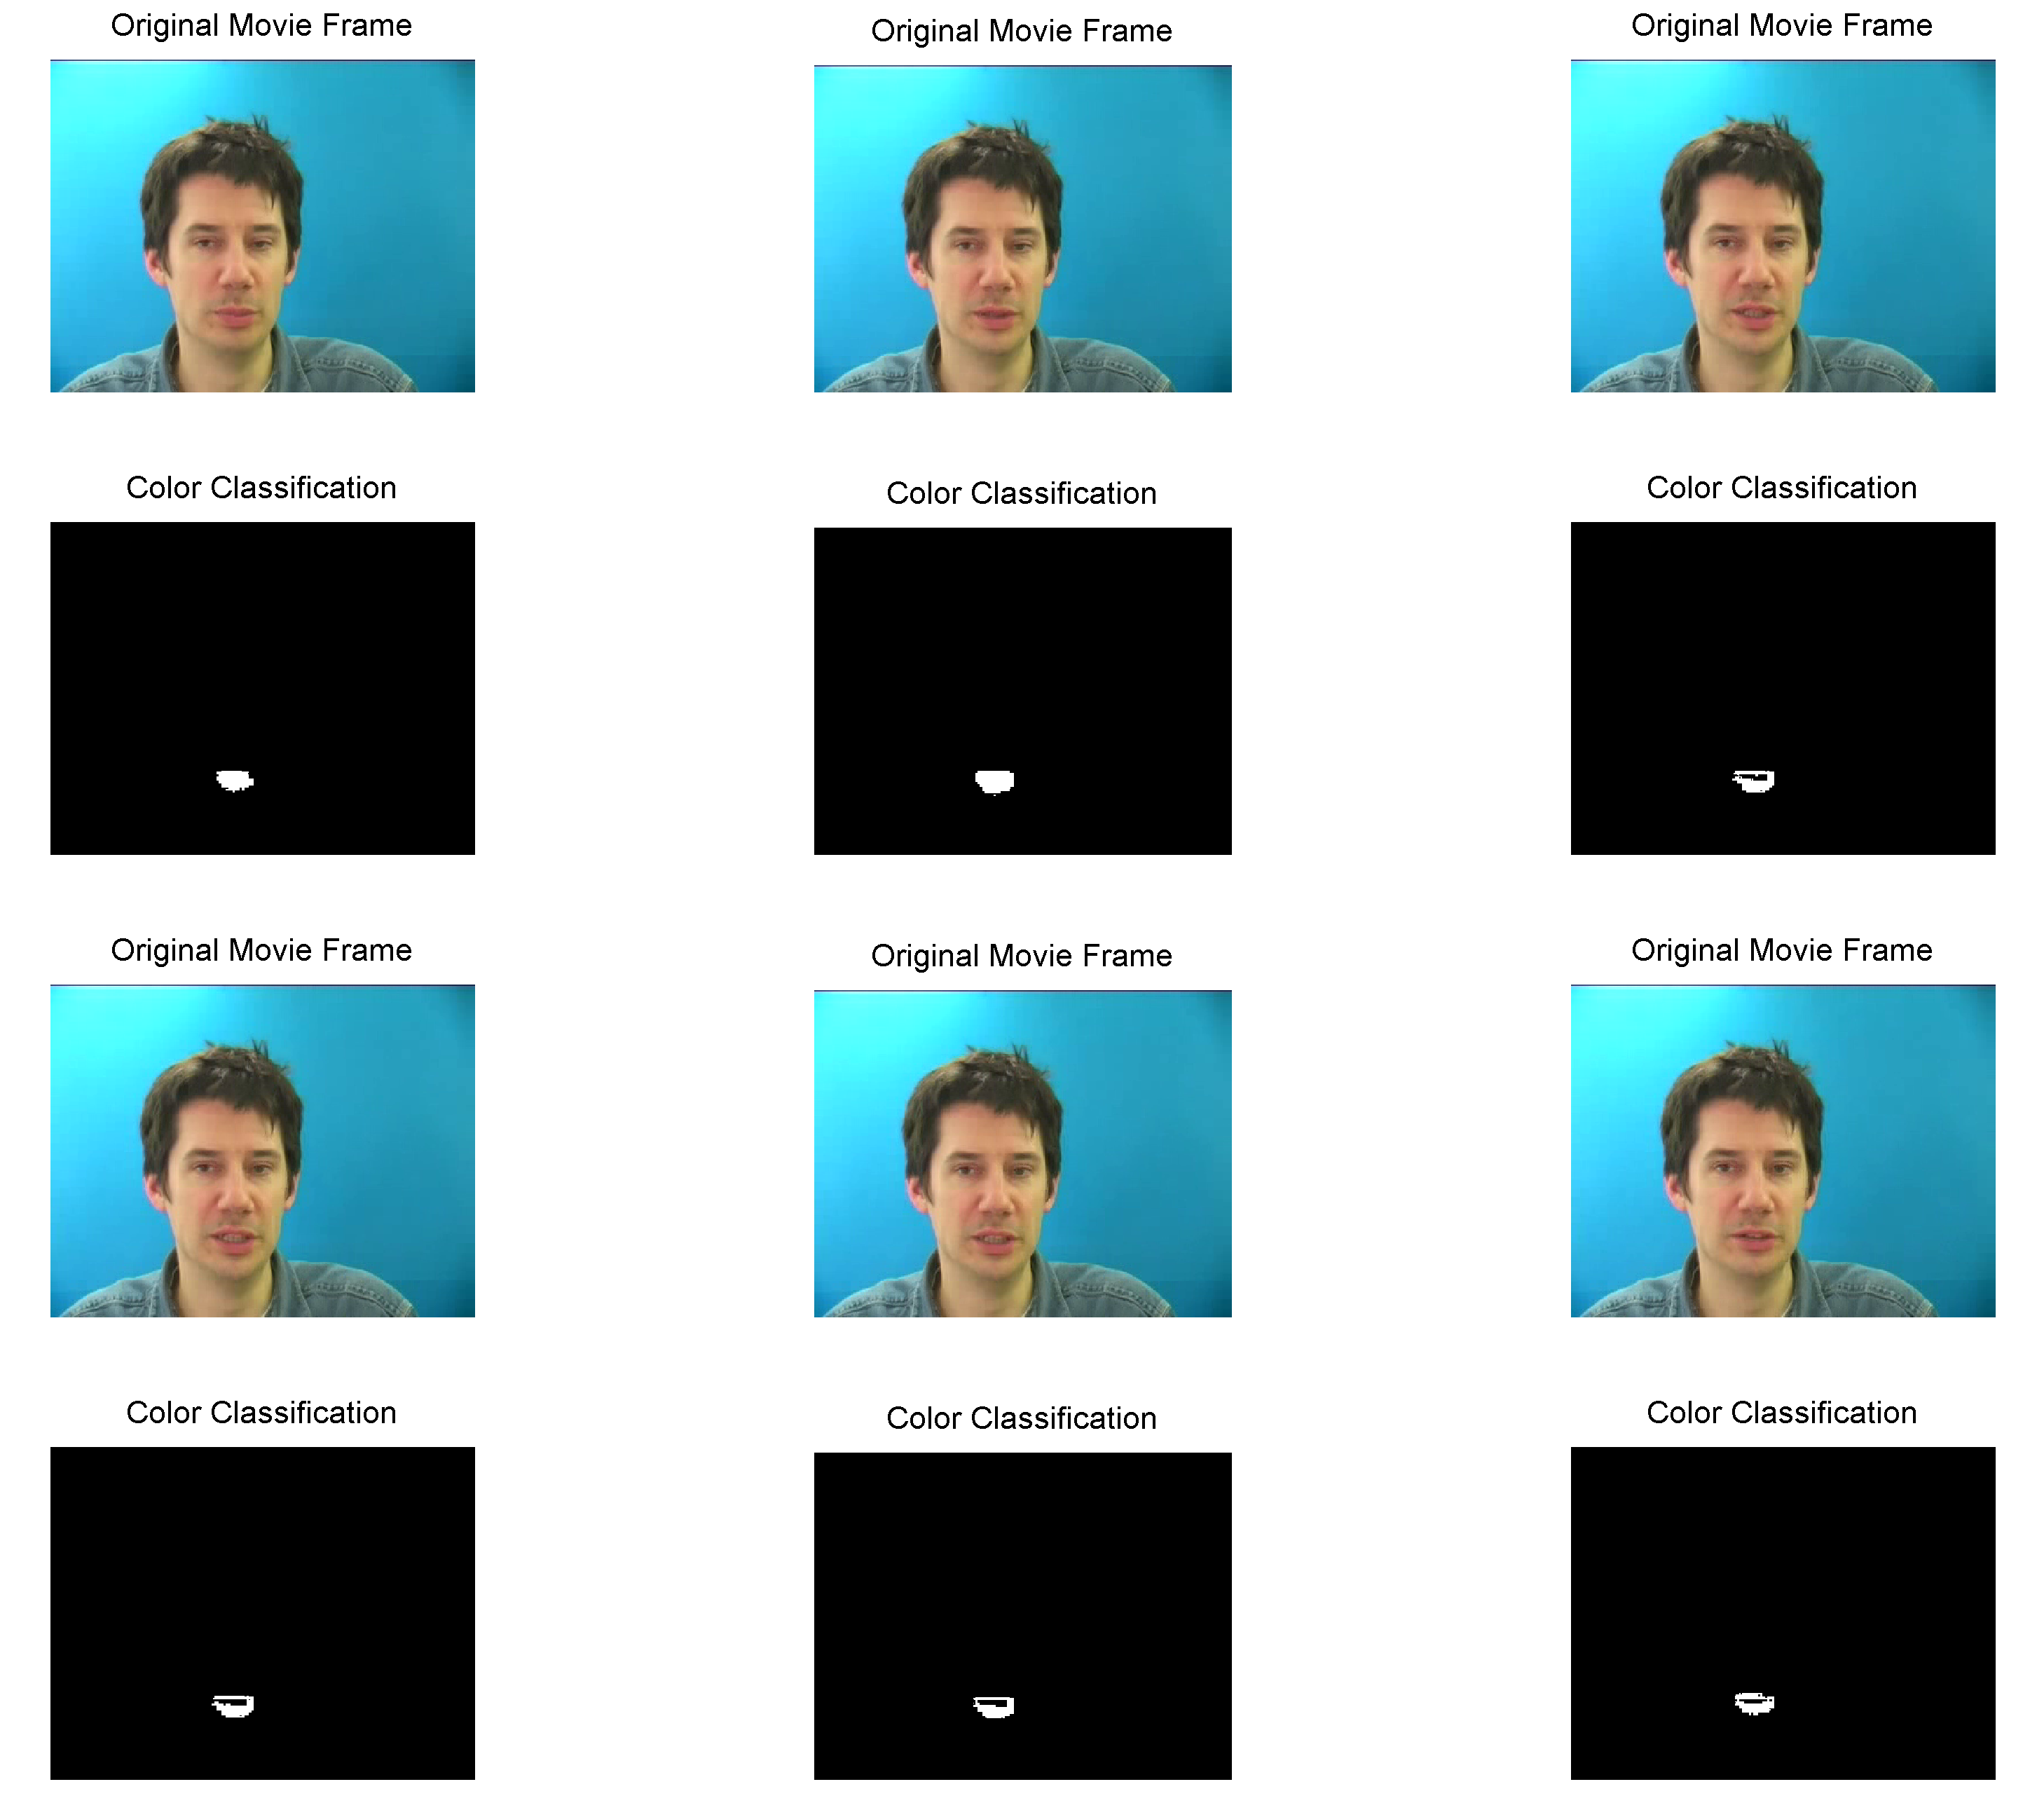
\includegraphics[width=1\textwidth]{color2.png}
	\caption{Color Classification for selected frames. Arguably the best overall method for capturing the movement of the lips.}
\end{figure}

\section*{Abstract}
The goal of this project is to develop a limited lip reading algorithm for a subset of the english language. We consider a scenario in which no audio information is available. We first develop a method for processing raw video and extracting the position of the lips in each frame. We then prepare the lip data for processing and classify the lips into visemes and phonemes. We then use Hidden Markov Models to predict the words the speaker is saying based on  the classification. We use the GRID audiovisual sentence corpus database for our study. 

\section{Introduction}
We consider 4 different algorithms for extracting the lip position. \begin{itemize}
  \item Active Contour Mask (Matlab built in)
\item Dynamic Mode Decomposition 
\item Edge Detection (Matlab built in)
\item Color Classification
\end{itemize}
We apply these techniques on a group of 1000 videos of a single speaker from the GRID audiovisual sentence corpus database. Each video is 3 second long and contains the speaker saying a number of nonsense phrases. The phrases spoken are chosen to convey a variety of sounds and therefore lip positions.



\section{Theoretical Development}
Lip reading is a complicated task and there are no "go-to" algorithms for detecting and tracking the position of an individual's lips. We can use Matlab's built in active contour and edge detection to hope to do background/foreground seperation on the video. We can also use DMD to do background/foreground seperation. The assumption is the speaker's face is stationary enough that it is possible to detect the lips as the foreground. In practice, this is not the case. We can also classify the pixel colors of the video frames and segment the lips based on the idea that the speaker's lip color is different from their skin color. For color classification, we can project the pixel color into the LAB color space to acheive better classification results. In either of these different strategies we also need to isolate the general mouth region of the speaker so that we will not also detect eyes, nose, etc.

\section{Algorithm Development}

The first step is to determine the general location of the mouth in each frame. Matlab has a built in facial recognition package ``Cascade Vision Detector'' which uses the Viola-Jones algorithm to detect the facial features of people. We use the Cascade Mouth detector to determine the location of the face in each frame of each movie. This algorithm is not perfect however and we often detect the eyes or chin of the subject in question. We filter out these false detections by looking at the position of the mouth. The speaker is in generally the same location in each movie so we know if a detected mouth position is too low or too high we can throw that region out. We refer to this detected mouth region as the \textit{initial mask}. We need a good initial mask in order to properly filter our results. Without knowing the general mouth region our algorithms will act on the whole face, but we consider only the lips for our project. Therefore, our real objective is to separate the lips from the mouth region.\par
Next we convert the image to grayscale. On the grayscale image we can apply Matlab's built in active contour and edge detection, as well as the DMD algorithm we develop in homework 4. We can experiment with the different segmentation types for Matlab's active contour and edge detection. For active contour, Chan-Vese gives poor results with irregular edges. Edge method for active contour gives smoother regions but irregular shapes. Active contour takes many iterations to properly converge and gives poor results. From the figures of active contour, we see the inconsistent lip region detected. Because we are trying to determine the changes in lip shape over time, active contour is not suitable because the results it produces vary too much. Additionally, because it is extremely slow, active contour is not ideal for our purposes. We need to process a large number of videos so a fast algorithm is preferable. If active contour was more computationally efficient it might be possible to use a large number of iterations for each frame in order to obtain a consistent result.  \par
 Matlab's built in edge detection has many different methods which produce different results. We consider using Canny, Prewitt and Sobel edge detection.Canny typically finds the ``strong'' edges whereas Sobel and Prewitt tend to pick out more detail in the image. We are really only interested in the lips, and ideally want only 1 contour, so we decide to use Canny edge detection. We want to detect the outside and inside edge of the lips, but all methods typically detect  the inside edge of the lip. When using Matlab's ``edge'', it is important to consider the threshold. Too low a threshold value will produce other features of the face and possibly noise. Too high a threshold and we will not pick out the entire lip. Therefore we decide to start at a high threshold value, and if we do not find a large enough edge, we lower the threshold and do the detection again. Typically we only need the lower the threshold once or twice. We set a minimum number of detected pixels in the edge to decide whether or not to automatically lower the threshold. Although this may seem expensive, in practice we only need to lower the threshold for certain frames, and so most of the time we only need to do the algorithm once.  Additionally, edge is much faster than active contour, so this method is still much faster than active contour, and gives more consistent results in well. Overall the Canny edge detection finds a good edge for the lips but it oftentimes only picks out part of the mouth or sometimes picks out other features around the mouth as well, like the chin or space between the nose and mouth.\par
 Next we use the DMD algorithm we developed in homework 4 to try foreground/background seperation. We find that the face moves too much, and there is too much variation in the speaker's skin around the mouth to properly use DMD. We detect many points that are not on the lip. While DMD is good at seperating the man's face from the background, it cannot accurately seperate the lips from mouth region. It might be possible to alter the brightness and contrast of the seperated image using DMD to obtain a better result, but it would still be too inconsistent to obtain good results for the rest of the project. \par
 Thus far, all of the methods discussed have acted on grayscale frames of the color movie. We now consider a technique for acting on the color frames. If we assume that the lips of the speaker have a distinct color from the rest of the speaker's mouth region (i.e. the skin, teeth, inside of the mouth) then we can determine the lip region by classifying the colors of the mouth region. It is possible to do this using the RGB values of each pixel. We instead represent each pixel with it's LAB color space values. The point of LAB colors  is that they match how human vision perceives colors. The L stands for lighting and AB are values corresponding to color. By classifying each pixel into one of up to 4 clusters based on it's AB values with a k-means algorithm, we can seperate the lips from the rest of the mouth region. The number of clusters created varies per frame because in some frames, the teeth and inner mouth can be grouped in their own clusters. Other frames, the speaker has their mouth closed so only 2 clusters are needed. We can differentiate between the clusters by looking at the calculated centroid positions of each cluster. It is determined experimentally that the lip region has the highest A color value, and it usually has the lowest B color value as well.  Color classification is fairly fast and accurate. It gives the thickness as well as the shape of the lips. It's only downside is that it often classifies the left and right sides of the lips into a different cluster. Color classification typically picks out an ellipse in the middle of the lips as opposed to the whole lip region. Overall, color classification is determined to give the most accurate results, and edge detection is a close second. In hindsight, it would have made much more sense to use a classification algorithm, like knn-search, instead of k-means. Although we choose the wrong algorithm to use our results are still acceptable. \par
 In general the best results come from either more computationally expensive or mathematically sophisticated techniques. For example, training a neural net to classify the lip region of each frame would probably be the most effective technique overall, but would be very computationally costly and require manually determining the lip region for training. Many papers in the literature consider fitting a vector to fit the lip region and then track the lips by moving points of the vector and measuring the change of shape. They then can compute the most likely shape by comparing it to known positions of the lip. This method relies more heavily on analysis but also requires manual training as well. In general, lip tracking is a classification problem where the goal is to classify the pixels that belong to the lip of the speaker. 

\end{document}

































